\documentclass[twocolumn]{article}
\usepackage{graphicx} % Required for inserting images
\usepackage{hyperref}
\usepackage{booktabs}
\usepackage{float}
\usepackage[margin=2cm]{geometry} 

\title{Text Classification of Milwaukee Bucks's Fan Comments on Reddit}
\author{John Collopy}
\date{April 30 2024}

\begin{document}

\maketitle


\begin{center}
\textbf{Abstract}
\end{center}

\begin{quote}
This project consisted of designing a Bernoulli Naive Bayes model, a Logistic Regression model, a Convolutional Neural Network, and a BERT model to classify Reddit comments in the r/MkeBucks subreddit according to thread label. The models were evaluated according to their F1 score, while precision and recall were analyzed as well. These metrics indicated that the Bernoulli Naive Bayes model performed best on both the validation and testing data; however, the model's relatively high number of false positive classifications speak both to the difficulties of classifying social media data as well as definitively determining the superiority of any model concerning this text classification problem.
\end{quote}

\section{Introduction}

The goal of this project was to evaluate the performances of different text classification methods on domain-specific social media data. The data used are comments from Milwaukee Bucks's fans in post-game Reddit threads from the subreddit r/MkeBucks, and models were used to predict whether a comment in a post-game thread followed a win or a loss. The data consisted of over 9,000 comments following 64 games, at which point the Milwaukee Bucks had a record of 41 wins and 23 losses. Classifying social media content can be difficult due to the use of informal language, lack of context, and ambiguity, and in this specific domain, there was concern that these problems might be exacerbated in a space of passionate fans. There are questions as to which methods best handle such difficulties, and so the project will consist of implementing and evaluating different text classification methods on the Reddit comments mentioned above. For this project, Bernoulli Naive Bayes, Logistic Regression, a Convolutional Neural Network, and a BERT model were used for the classifications. The respective performances of these different methods might be of use to others searching to perform text classification on domain-specific social media content.

\section{Background/Related Work}

\subsection{Paper 1}

Kanish Shah and other contributors in their paper, "A comparative analysis of logistic regression, random forest and KNN models for the text classification." analyze the performances of different machine learning approaches to text classification problems. The data used in their project is BBC news articles. The project in this analysis also compares different approaches to text classification, but specifically in regards to social media data, rather than news articles.

\subsection{Paper 2}

Santiago González-Carvajal and Eduardo C. Garrido-Merchán in their paper, "Comparing BERT against traditional machine learning text classification." explore the efficacy of BERT models in text classification. They argue that BERT offers a flexibility that other models cannot offer in this sort of problem. The authors used an IMBD movie review dataset for their study. While this project will explore the performances of BERT on text classification, the project will evaluate the performance of BERT on a very different type of text data, and thus could yield drastically different results.

\subsection{Paper 3}

Shaomin Zheng and Meng Yang in their paper "A new method of improving bert for text classification." argue for the superiority for BERT models in text classification. That being said, they claim that shortcomings exists in BERT models, particularly in their inability to recognize context in longer text data. It is to be seen if this shortcoming exists when classifying social media data.

\subsection{Paper 4}

David Rogers and contributors in their paper, "Real-time text classification of user-generated content on social media: Systematic review." speak to the superior performance of neural networks over traditional machine learning techniques in text classification. In their reasearch, they studied social media data from a multitude of sites. It is in this respect that my project differs from theirs, as I analyze social media data from a specific site. It is to be seen whether neural networks outperform traditional machine learning techniques in my project.

\subsection{Paper 5}

Hemant Purohit and contributors in their paper, "Intent classification of short-text on social media." discuss the difficulties discerning intent in social media text data. This task will be a challenge in my analysis, as understanding intent will allow for more accurate classifications. However, this project is not necessary classifying with respect to intent, but with respect to a thread label that might reflect intent.

\section{Model Building Approach}
\subsection{Naive Bayes}
The Bernoulli Naive Bayes model was built using Python's \texttt{scikit-learn} library. The comments were tokenized using the \texttt{CountVectorizer()}, adhering to the Bag of Words model framework. For this model, the Reddit comments were stemmed, stopwords were removed, and non-alphanumeric characters were removed. A simple modification was made to the default settings of \texttt{CountVectorizer()} and Bernoulli Naive Bayes in \texttt{scikit-learn} by allowing the model to capture bi-grams, as while the goal was to keep the Naive Bayes model simple, accounting for bi-grams made the model more able to capture language patterns within the data.

\subsection{Logistic Regression}
The Logistic Regression model was built using Python's \texttt{scikit-learn} library. The comments were tokenized using the \texttt{CountVectorizer()}, adhering to the Bag of Words model framework. For this model, the Reddit comments were stemmed, stopwords were removed, and non alphanumeric characters were removed. A simple modification was made to the default settings of \texttt{CountVectorizer()} and Logistic Regression in \texttt{scikit-learn} by allowing the model to capture bi-grams, as while the goal was to keep the Logistic Regression model simple, accounting for bi-grams made the model more able to capture language patterns within the data.

\subsection{Convolutional Neural Network}
The Convolutional Neural Network was constructed using \texttt{TensorFlow} and \texttt{Keras} libraries. For this model, nonalphanumeric characters were removed, but the comments were not stemmed, and stopwords were left in, as it was anticipated that the Neural Network would better be able to navigate these features better than the Naive Bayes and Logistic Regression models. The model was designed in a function with customizable hyperparameters such as number of filters, kernel size, number of dense layer neurons, learning rate, and dropout rate. The model's architecture consists of an embedding layer that maps text to dense vectors, a convolutional layer for feature extraction with a ReLU activation function, a max pooling layer to reduce dimensionality, a flattening step, and dense layers with L2 regularization targeted at binary classification through a sigmoid activation function. A major concern when designing this CNN was overfitting, and so an early stopping callback was implemented in the model. Then, a grid of the hyperparameters mentioned above was iterated over in order to determine the optimal model design. The hyperparameter-tuning indicated that the best model had hyperparameters: \texttt{filters = 48}, \texttt{kernel size = 4}, \texttt{number of dense layers = 40}, \texttt{learning rate = 0.001}, and \texttt{dropout rate = 0.6}.

Below are the formulas for the activation functions:

\begin{center}
ReLU: \(f(x) = \max(0, x)\)
\end{center}

\begin{center}
Sigmoid: \( f(x) = (1 + e^{-x})^{-1} \)
\end{center}

As mentioned, and early stopping callback was implemented, and below is a visualization of the training and validation accuracy over the number of epochs for which it was trained.

\begin{figure}[H]
    \centering
    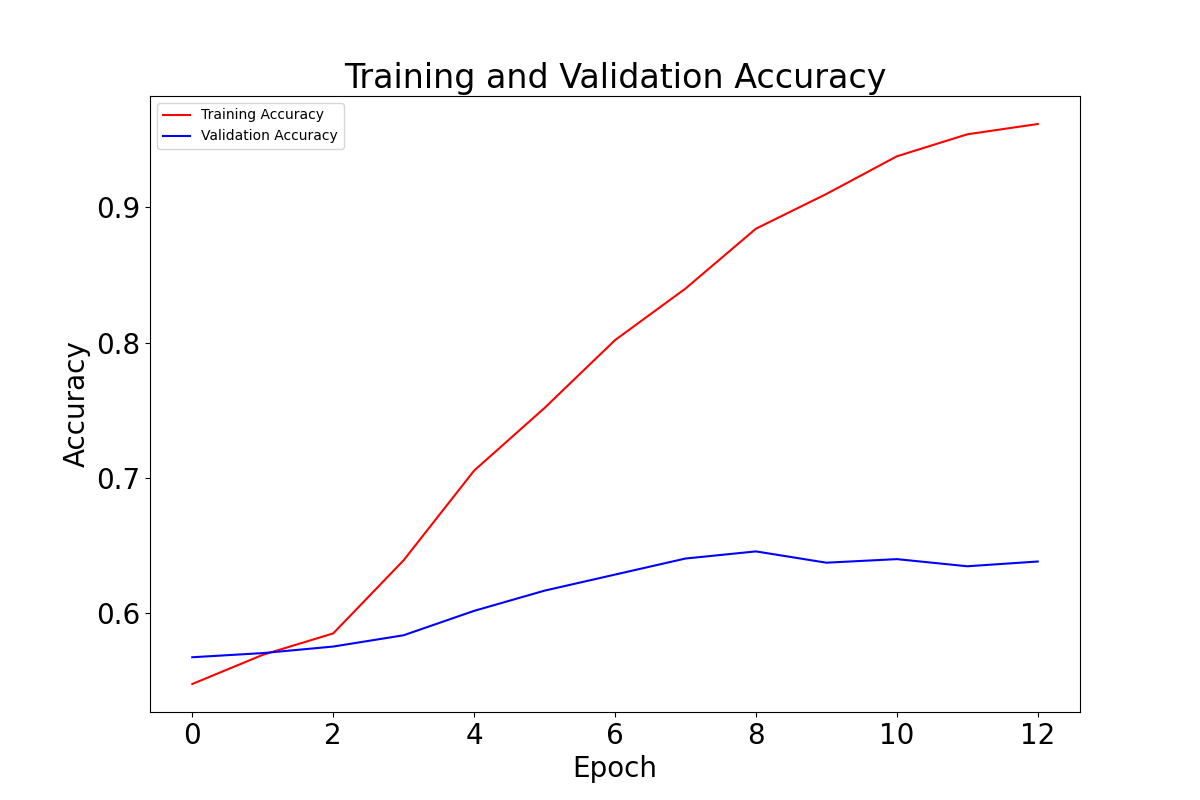
\includegraphics[width=\linewidth]{accuracy_plot.png}
    \caption{Training vs. Validation Accuracy CNN}
\end{figure}

As seen in the figure, the validation accuracy stopped growing at around 8 epochs, at which point the model stopped its training. Thus, overfitting concerns were addressed.

\subsection{BERT Model}
The pre-trained BERT model selected for this task was the MiniBERT model from Python's HuggingFace library. This model was chosen largely due to the limited computational resources available for this project, as MiniBERT is smaller and faster than other BERT models. 

The optimizer selected was Adam with a standard learning rate of `5e-5`. The training loop for this model consisted of a forward pass, in which a batch of size 30 was passed into the model, and a backward pass, in which the gradients were computed and model parameters updated according to the magnitude of the Cross Entropy loss. Below is a visual showing the training vs. validation accuracy over 6 epochs.

\begin{figure}[H]
    \centering
    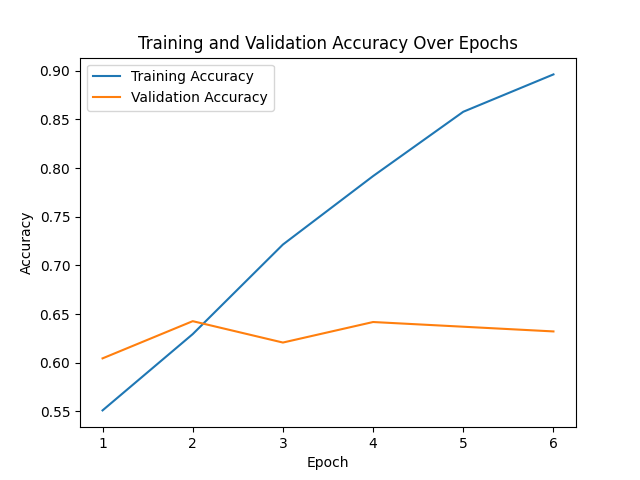
\includegraphics[width=\linewidth]{bert_accuracy_plot.png}
    \caption{Training vs. Validation Accuracy BERT}
\end{figure}

Interestingly, the validation accuracy starts how higher than the training accuracy, but this changes quite quickly. This plot illustrates that extreme overfitting is avoided in training, as the training accuracy is not dramatically higher than validation accuracy.

\section{Experiments}

\subsection{Model Performances on Training Data}

The following subsections outline the respective performances of the different models on the training data.

\subsubsection{Naive Bayes}
The initial model built was a Bernoulli Naive Bayes model. After fitting it to the training data, below are some performance metrics on the validation data:

\begin{table}[H]
\centering % This centers the table
\caption{\textbf{Naive Bayes on Validation Data}} 

\begin{tabular}{ccc} 
\toprule
Precision & Recall & F1 \\ 
\midrule
0.574 & 0.943 & 0.714 \\
\bottomrule
\end{tabular}
\end{table}

As seen in the table above, there is a stark difference between the model's Precision and Recall scores, which indicates that the model yields a high number of False Positive classifications. This indicates that the model frequently predicts losing comments as winning ones, while rarely misclassifying winning comments as losing ones. This is evident in the confusion matrix below.

\begin{figure}[H]
    \centering
    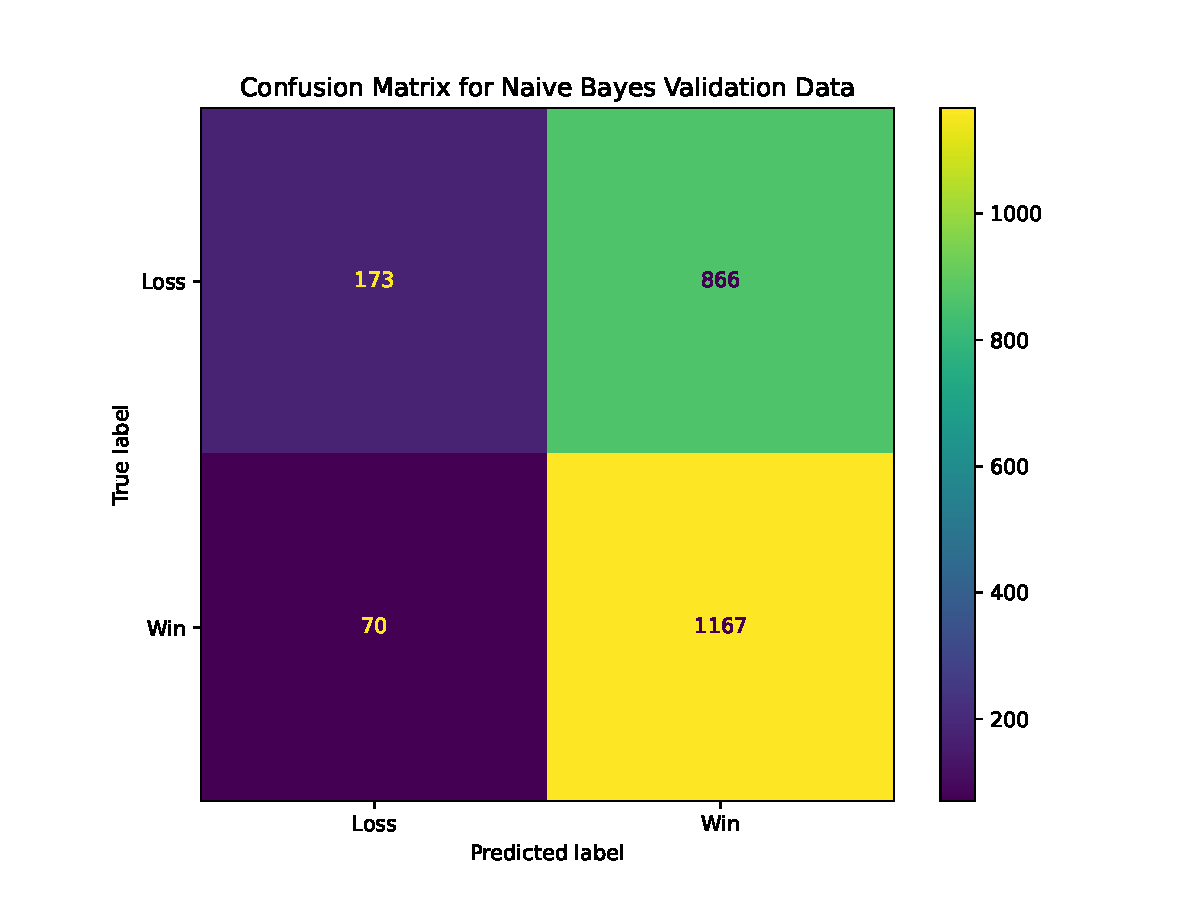
\includegraphics[width=\linewidth]{nbv_confusion_matrix.pdf}
    \caption{Confusion Matrix For N.B. Validation Data}
\end{figure}

The high number of False Positives in the confusion matrix above was concerning, but the low number of False Negatives helped offset this shortcoming, and this is reflected in the F1 score.

\subsubsection{Logistic Regression}

The next model built was a Logistic Regression model. After training it on the training data, below are some performance metrics on the validation data:

\begin{table}[H]
\centering % This centers the table
\caption{\textbf{Logistic Regression on Validation Data}} 

\begin{tabular}{ccc} 
\toprule
Precision & Recall & F1 \\ 
\midrule
0.665 & 0.733 & 0.698 \\
\bottomrule
\end{tabular}
\end{table}

Interestingly, while there is still a difference between Precision and Recall, the gap is not as wide as that in the Naive Bayes model. The precision is higher, while the recall is much lower, which indicates that Logistic Regression better handles predicting losses while mishandling wins more frequently. This can be seen in the confusion matrix below.

\begin{figure}[H]
    \centering
    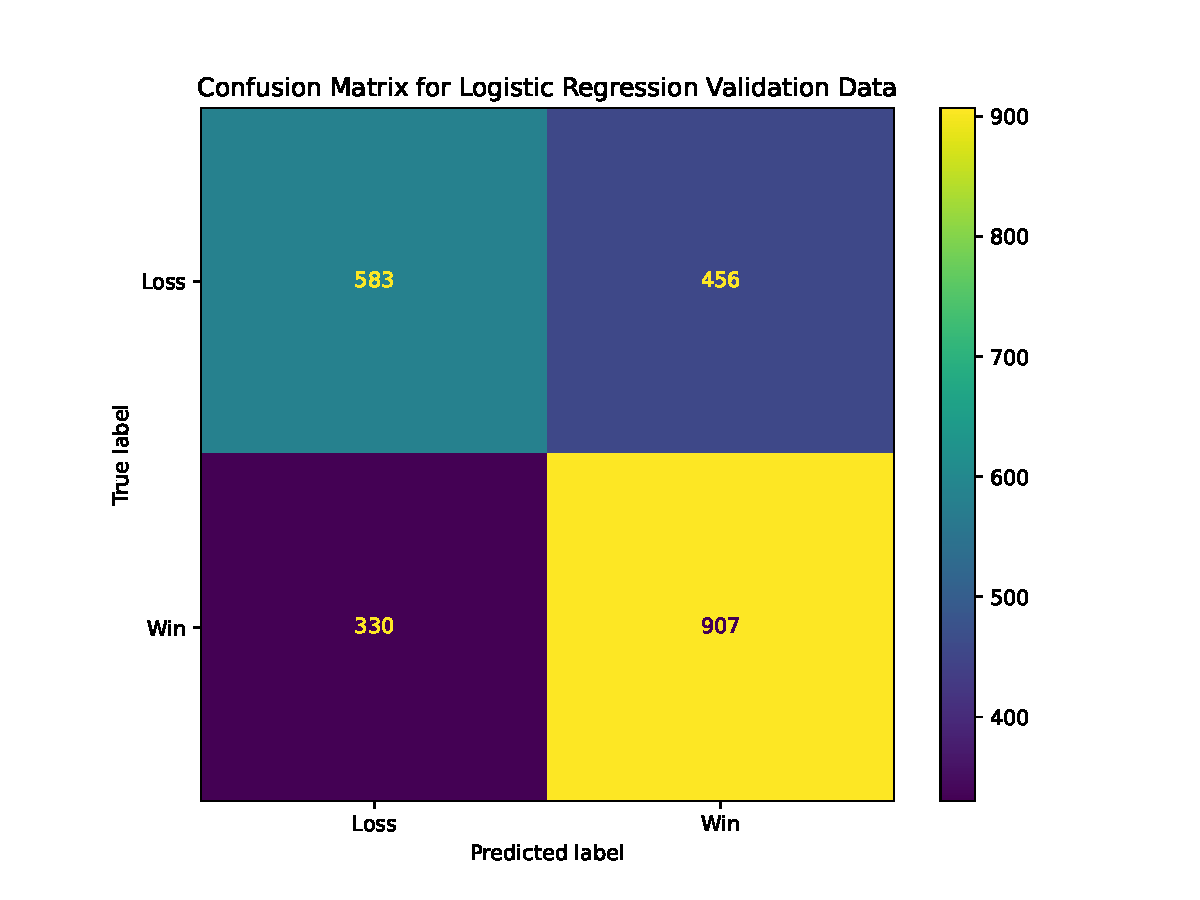
\includegraphics[width=\linewidth]{lrv_confusion_matrix.pdf}
    \caption{Confusion Matrix for L.R. on Validation Data}
\end{figure}

Although it handles certain classifications better than the Naive Bayes (as seen above in the number of True Negatives), due to its lower F1 score, it is so far the worst performing model.

\subsubsection{Convolutional Neural Network}
Next, a Convolutional Neural Network was designed. After training it on the training data, below are some performance metrics on the validation data. 

\begin{table}[H]
\centering % This centers the table
\caption{\textbf{CNN on Training Data}} 

\begin{tabular}{ccc} 
\toprule
Precision & Recall & F1 \\ 
\midrule
0.641 & 0.771 & 0.7 \\
\bottomrule
\end{tabular}
\end{table}

This model performs quite similarly to the Logistic Regression model, although the F1 score is slightly higher. Their respective precision and recall scores are quite close, indicating that the Convolutional Neural Network handles predicting losses better than the Naive Bayes model, while failing to predict wins as favorably. This can also be seen in the Confusion Matrix below.

\begin{figure}[H]
    \centering
    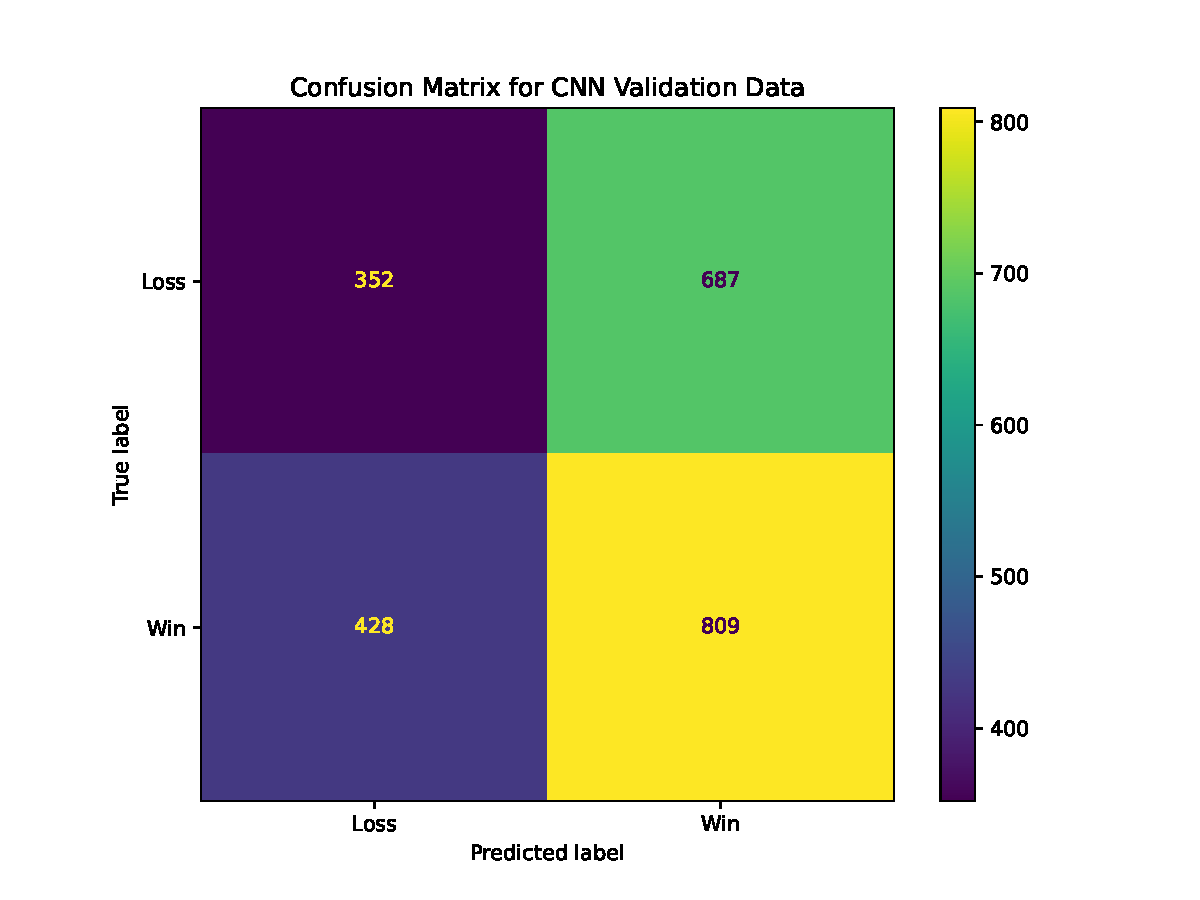
\includegraphics[width=\linewidth]{cnnv_confusion_matrix.pdf}
    \caption{Confusion Matrix For CNN Validation Data}
\end{figure}

Essentially, similar to the Logistic Regression, it does handle some classifications better than the Naive Bayes (as seen above in the number of True Negatives), yet it still has a lower F1 score.

\subsubsection{BERT Model}

Next, a BERT was designed. After training it on the training data, below are some performance metrics on the validation data.

\begin{table}[H]
\centering % This centers the table
\caption{\textbf{BERT on Training Data}} 

\begin{tabular}{ccc} 
\toprule
Precision & Recall & F1 \\ 
\midrule
0.685 & 0.637 & 0.66 \\
\bottomrule
\end{tabular}
\end{table}

These metrics stand out when compared to all other models, as the precision is higher than the recall. Thus, this is the first model that handles losing comments better than wins. This can be seen in the confusion matrix below.

\begin{figure}[H]
    \centering
    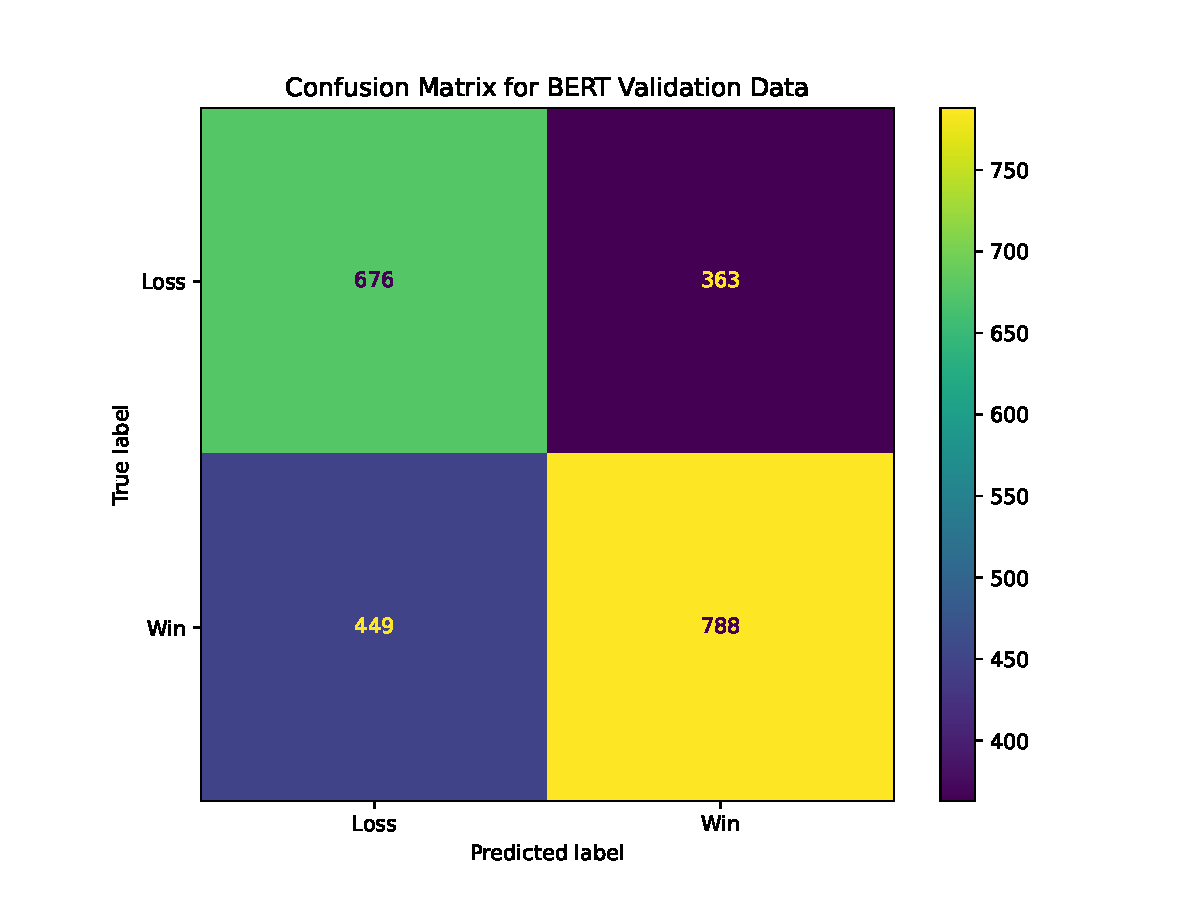
\includegraphics[width=\linewidth]{bertv_confusion_matrix.pdf}
    \caption{Confusion Matrix for BERT Training Data}
\end{figure}

Although this model stands out, given its low F1 score, it the worst performing model on the validation data.

In this initial analysis, the Naive Bayes model performed best on the validation data, although some concerns about its performance were raised. An exploration of the testing data was necessary to determine if trends in validation evaluation persisted.

\subsection{Model Performances on Test Data}

The following subsections outline the respective performances of the different models on the testing data.

\subsubsection{Naive Bayes}

Below are some performance metrics from the Naive Bayes model on the test data:

\begin{table}[H]
\centering % This centers the table
\caption{\textbf{Naive Bayes on Testing Data}} 

\begin{tabular}{ccc} 
\toprule
Precision & Recall & F1 \\ 
\midrule
0.574 & 0.953 & 0.717 \\
\bottomrule
\end{tabular}
\end{table}

Below is the confusion matrix to supplement the metrics above.

\begin{figure}[H]
    \centering
    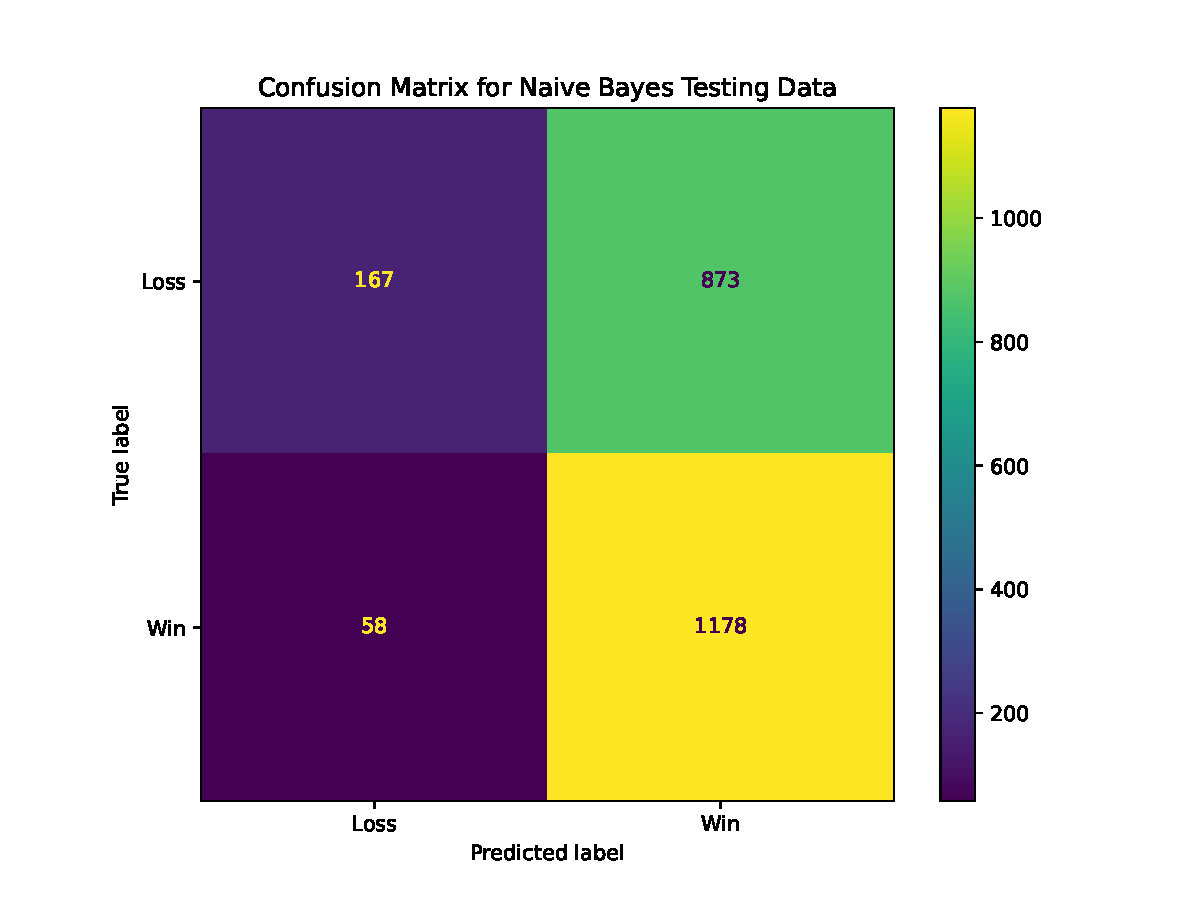
\includegraphics[width=\linewidth]{nbt_confusion_matrix.pdf}
    \caption{Confusion Matrix for N.B. Testing Data}
\end{figure}

Many of the same problems exist in the Naive Bayes' respective performances on the validation and testing data. The stark difference between precision and recall remains, although there are slight improvements in precision, recall, and F1. Essentially, it is clear that the Naive Bayes yields a high F1 score, but it struggles to correctly classify comments from losing post-game threads.

\subsubsection{Logistic Regression}
Below are some performance metrics from the Logistic Regression model on the test data:

\begin{table}[H]
\centering % This centers the table
\caption{\textbf{Logistic Regression on Testing Data}} 

\begin{tabular}{ccc} 
\toprule
Precision & Recall & F1 \\ 
\midrule
0.661 & 0.749 & 0.703 \\
\bottomrule
\end{tabular}
\end{table}

Many of the same trends appear in the Logistic Regression's respective performances on the validation and testing data. Given the higher recall score, the model seems to handle predicting wins than losses. However, when compared to the Naive Bayes model, it predicts Losses better and Wins more poorly. The F1 score is slightly lower. The magnitude of this trend can be seen in the confusion matrix below.

\begin{figure}[H]
    \centering
    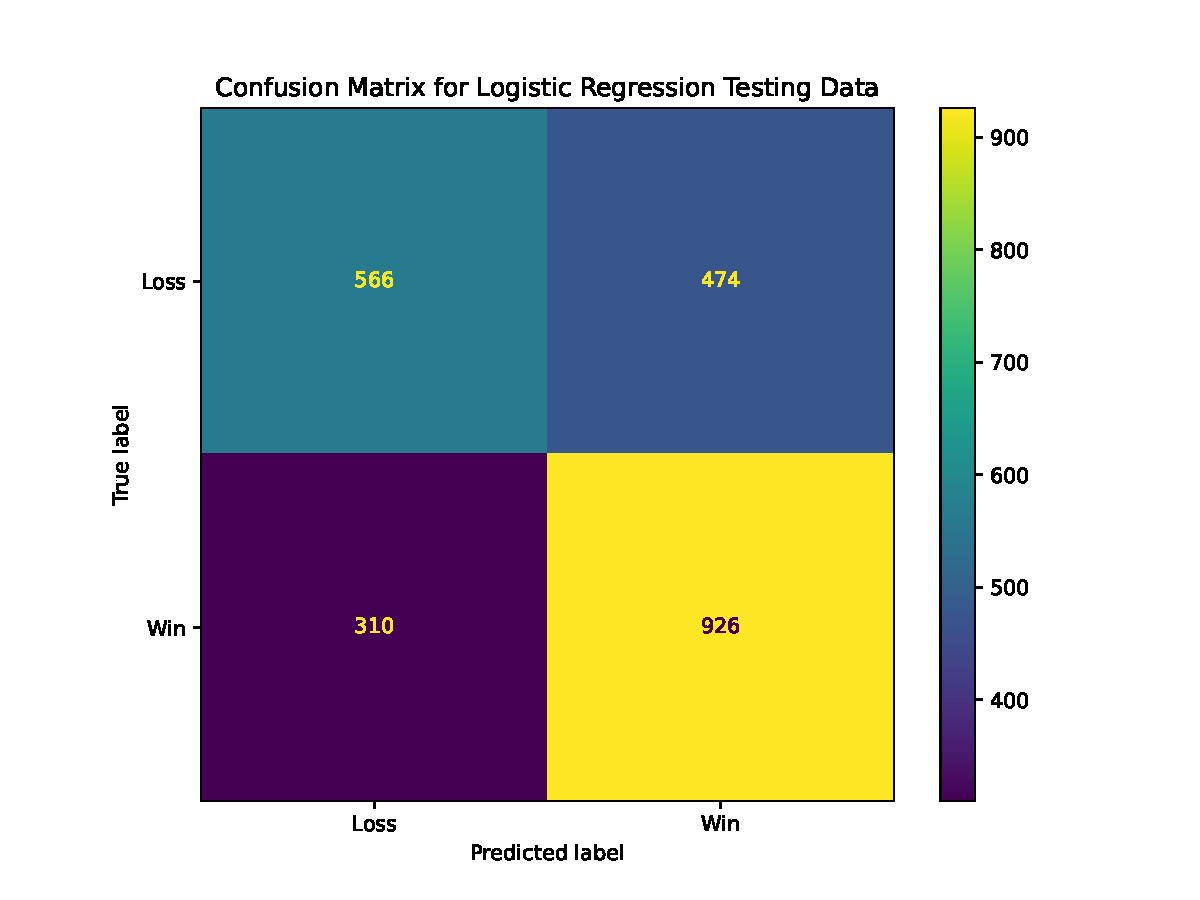
\includegraphics[width=\linewidth]{lrt_confusion_matrix.pdf}
    \caption{Confusion Matrix for L.R Testing Data}
\end{figure}

Just as in the validation set, the Logistic Regression does not earn as high of performance metrics as the Naive Bayes. However, it does clearly perform more strongly in different areas of the data than the Naive Bayes, and the lower number of false positives in the confusion matrix highlights this notion..

\subsubsection{Convolutional Neural Network}
Below are some performance metrics from the Convolutional Neural Network on the test data:
\begin{table}[H]
\centering % This centers the table
\caption{\textbf{CNN on Testing Data}} 

\begin{tabular}{ccc} 
\toprule
Precision & Recall & F1 \\ 
\midrule
0.665 & 0.733 & 0.698 \\
\bottomrule
\end{tabular}
\end{table}

Many of the same trends appear in the CNN's respective performances on the validation and testing data. Given the higher recall score, the model seems to handle predicting wins than losses, just as the Logistic Regression model does. However, when compared to the Naive Bayes model, it predicts losses better and wins more poorly, just as the Logistic Regression model does. The F1 score is slightly lower than it is in the training section. The magnitude of this trend can be seen in the confusion matrix below.

\begin{figure}[H]
    \centering
    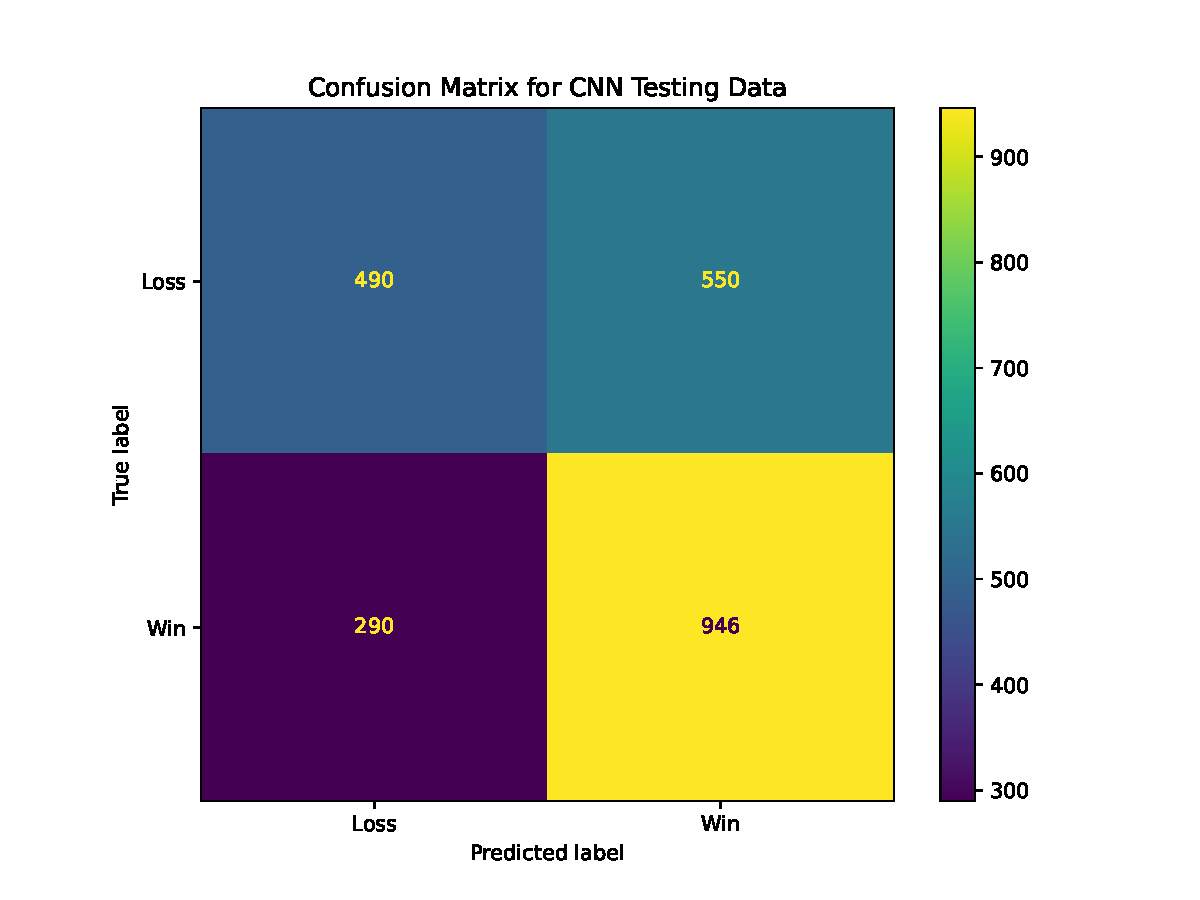
\includegraphics[width=\linewidth]{cnnt_confusion_matrix.pdf}
    \caption{Confusion Matrix for CNN Testing Data}
\end{figure}

As seen in the confusion matrix above, the CNN does perform better in some areas of the data than the Naive Bayes model, but since the scoring criterion for this analysis is F1 score, we cannot say that it is the superior model in this task.

\subsubsection{BERT Model}

Below are some performance metrics from the BERT model on the testing data:

\begin{table}[H]
\centering % This centers the table
\caption{\textbf{BERT on Testing Data}} 

\begin{tabular}{ccc} 
\toprule
Precision & Recall & F1 \\ 
\midrule
0.674 & 0.633 & 0.653 \\
\bottomrule
\end{tabular}
\end{table}

These metrics still stand out when compared to all other models, as the precision is higher than the recall. Even what evaluated on the testing data, the precision is still higher than recall, thus it is the only model whose relative strength is avoiding False Positive classifications. This is also seen clearly in the confusion matrix below.

\begin{figure}[H]
    \centering
    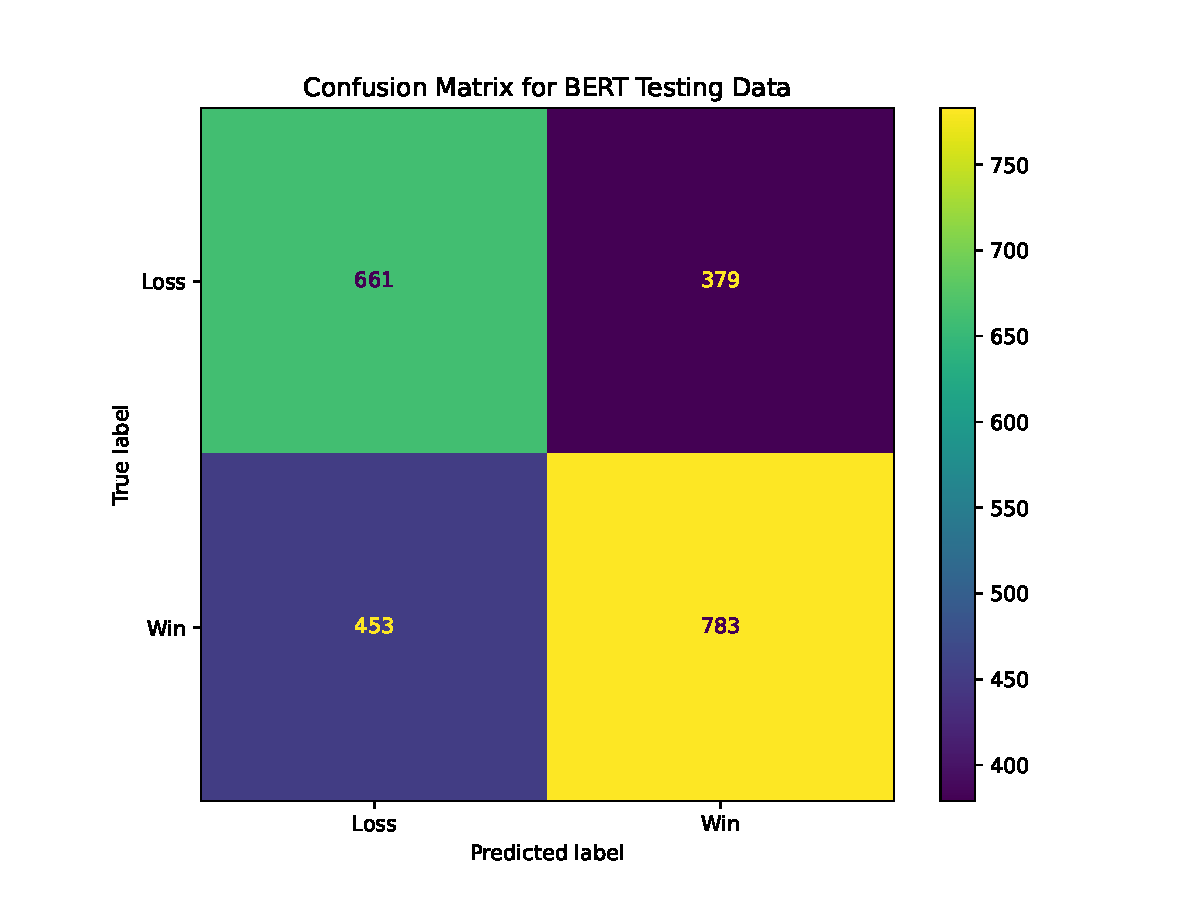
\includegraphics[width=\linewidth]{bertt_confusion_matrix.pdf}
    \caption{Confusion Matrix for BERT Testing Data}
\end{figure}

The metrics and confusion matrix above indicate that the BERT model's relative strength is correctly identifying comments that come from losing threads, unlike every other model.

\subsection{Error Analysis}

Perhaps the most striking result in the model evaluations was the low Precision score of the Naive Bayes, as it struggled to correctly predict comments that followed losses. Thus, it is worth looking at some comments that the Naive Bayes model incorrectly predicted as a winning comment and the Logistic Regression, CNN, and BERT model correctly classified. Below is one of these comments:

\begin{center}
\textit{Dame is checked out and is perpetually lazy, apathetic, and downright stupid on the court. It’s miserable to watch. I miss Jrue, and Khris is better than Dame right now}
\end{center}

This comment clearly is expressing some negative sentiment towards the Damian Lillard, one of their highest performing players, yet the Naive Bayes model predicted that it would be in a winning thread. Let's see some of the associated probabilities with each word following a loss:

\begin{table}[H]
\centering
\begin{tabular}{l r}
\hline
Word & Probability \\
\hline
dame & 0.4727 \\
check & 0.3103 \\
perpetu & 0.5000 \\
lazi & 0.5000 \\
stupid & 0.6087 \\
court & 0.4726 \\
miser & 0.5556 \\
watch & 0.5420 \\
miss & 0.5689 \\
jrue & 0.5800 \\
khri & 0.4045 \\
better & 0.4494 \\
right & 0.5504 \\
\hline
\end{tabular}
\caption{Word Probabilities}
\label{tab:word_probabilities}
\end{table}

As seen in the table above, while there are more words associated with losing, the word "check" as a very low association with losing, which is likely why Naive Bayes classified it as a win. Now, here are the coefficients for the Logistic Regression:

\begin{table}[H]
\centering
\begin{tabular}{l r}
\hline
Word & Coefficient \\
\hline
dame & -0.1701 \\
check & 0.2474 \\
perpetu & -0.0280 \\
lazi & -0.2384 \\
stupid & -0.6631 \\
court & 0.1460 \\
miser & 0.1129 \\
watch & -0.2534 \\
miss & -0.4716 \\
jrue & -0.3370 \\
khri & 0.3443 \\
better & 0.1552 \\
right & -0.2622 \\
\hline
\end{tabular}
\caption{Word Coefficients}
\label{tab:word_coefficients}
\end{table}

Unlike in the Naive Bayes model, more of the words have losing associations, and words like "stupid" and "miss" have quite large negative coefficients, which explains the classification of the Logistic Regression model, which happens to be correct.

As mentioned earlier, the Naive Bayes model does a very good job compared to the other models as correctly classifying comments from winning post-game threads. Thus, it is worth looking at an example that only it got correct. Here is such an example:

\begin{center}
\textit{Malik is playing well, sending him to the bench now will throw him off}
\end{center}

This is a very interesting example, as it compliments a player, but Logistic Regression, the Neural Network, and BERT model all incorrectly classified it as a losing comment. Here is a simple breakdown as to why by comparing some measurements from the Naive Bayes and Logistic Regression. The Logistic Regression model assigns negative coefficients to every word in the sentence except "sending", and thus it classifies the comment as a losing one. Below are the coefficients:

\begin{table}[H]
\centering
\begin{tabular}{l r}
\textit{Word} & \textit{Coefficient} \\ \hline
malik & -0.5407 \\
play & -0.0569 \\
well & -0.2482 \\
send & 0.4619 \\
bench & -0.3270 \\
throw & -0.0845 \\
\hline
\end{tabular}
\caption{Word Coefficients}
\label{tab:word_coefficients}
\end{table}

On the other hand, the Naive Bayes model weakly associates "Malik", "playing", and "well" with losing, while it associates "sending", "bench", and "throwing" all more strongly with winning. Below are the probabilities of each word given a  win:

\begin{table}[H]
\centering
\begin{tabular}{l r}
\textit{Word} & \textit{Probability} \\ \hline
malik & 0.4348 \\
play & 0.4826 \\
well & 0.4767 \\
send & 0.6429 \\
bench & 0.5251 \\
throw & 0.5133 \\
\hline
\end{tabular}
\caption{Word Coefficients}
\label{tab:word_probabilities}
\end{table}

Thus, the different word assessments explain the different classifications. These different results speak to the difficulties in this task and how slightly different word evaluations lead to different results. Both comments above are relatively short, and perhaps more of an in-depth assessment on the part of the user would improve model performances and fewer differences between model results.

\section{Conclusions}
The main insight drawn from this analysis is the wide performance scope of the models. The Naive Bayes model had a very high recall score and a shockingly low precision score, while the BERT model had a very low recall score. While the Naive Bayes seemingly handled the winning labels very well, it would be interesting to see if this would hold across different NBA subreddits. As the scope of this project only pertains to a single subreddit, it would be interesting to evaluate the performances of these models across different subreddits for different NBA teams. As the Milwaukee Bucks won significantly more games than they lost, the nature of the comments in a subreddit of a losing team would likely be considerably different. Thus, the relative performances would likely change when used on different data, such as comments from the San Antonio Spurs subreddit. 

Essentially, this project does not yield definite insights regarding the general performances of these models on text classification, as this project's scope is rather niche. However, it was found that the traditional Bernoulli Naive Bayes method performed best, although only slightly and with legitimate shortcomings. On a different dataset, it is entirely possible that a different model would yield better metrics.


\section{References}
\bibliography{references}
\bibliographystyle{acl_natbib}

1. Shah, Kanish, et al. "A comparative analysis of logistic regression, random forest and KNN models for the text classification." Augmented Human Research 5 (2020): 1-16. \href{https://link.springer.com/article/10.1007/s41133-020-00032-0}{Link}


2. González-Carvajal, Santiago, and Eduardo C. Garrido-Merchán. "Comparing BERT against traditional machine learning text classification." arXiv preprint arXiv:2005.13012(2020). \href{https://arxiv.org/abs/2005.13012}{Link}


3. Zheng, Shaomin, and Meng Yang. "A new method of improving bert for text classification." Intelligence Science and Big Data Engineering. Big Data and Machine Learning: 9th International Conference, IScIDE 2019, Nanjing, China, October 17–20, 2019, Proceedings, Part II 9. Springer International Publishing, 2019. \href{https://link.springer.com/chapter/10.1007/978-3-030-36204-1_37}{Link}


4. Rogers, David, et al. "Real-time text classification of user-generated content on social media: Systematic review." IEEE Transactions on Computational Social Systems 9.4 (2021): 1154-1166. \href{https://ieeexplore.ieee.org/abstract/document/9585425}{Link}


5. Purohit, Hemant, et al. "Intent classification of short-text on social media." 2015 ieee international conference on smart city/socialcom/sustaincom (smartcity). IEEE, 2015. \href{https://ieeexplore.ieee.org/abstract/document/7463729}{Link}

\section{Screenshots}

Below are screenshots from my demo. The demo takes in a comment as input, and predicts whether the comment would be posted following a win or a loss according to the selected model. I attempted to draft a comment with some ambiguity. Here is the selected comment: "This team extremely is talented, but I am worried about the three point shooting, and I am skeptical going forward."

The Naive Bayes model classifies this comment as a "Win" with "Confidence" = 68.28%.

\begin{figure}[H]
    \centering
    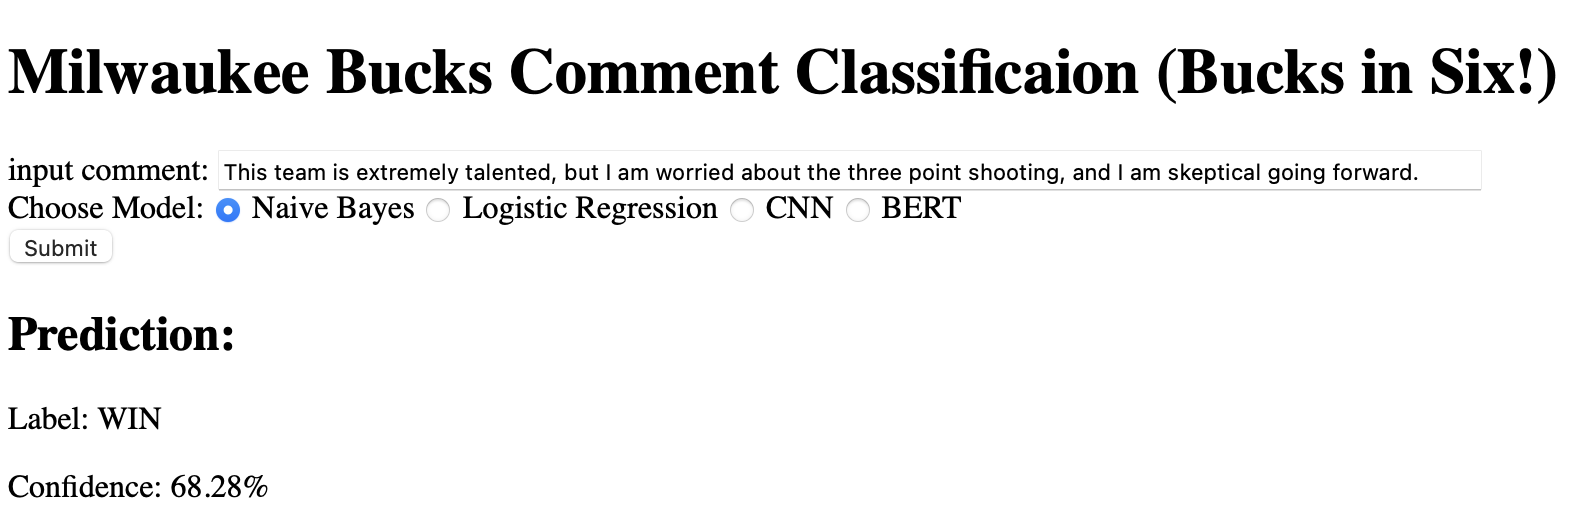
\includegraphics[width=\linewidth]{NBDEMO.png}
    \caption{Naive Bayes Demo}
\end{figure}

The Logistic Regression model classifies this comment as a "Loss" with "Confidence" = 51.92%.

\begin{figure}[H]
    \centering
    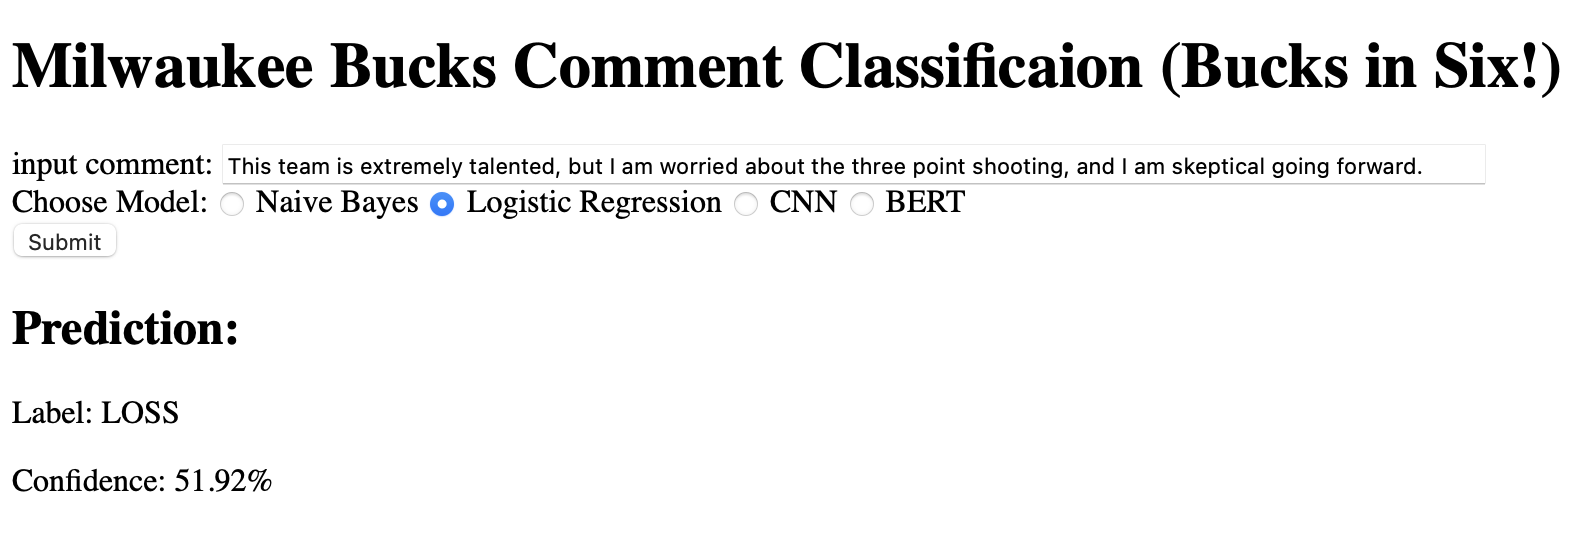
\includegraphics[width=\linewidth]{LRDEMO.png}
    \caption{Logistic Regression Demo}
\end{figure}

The CNN model classifies this comment as a "Win" with "Confidence" = 53.72%.

\begin{figure}[H]
    \centering
    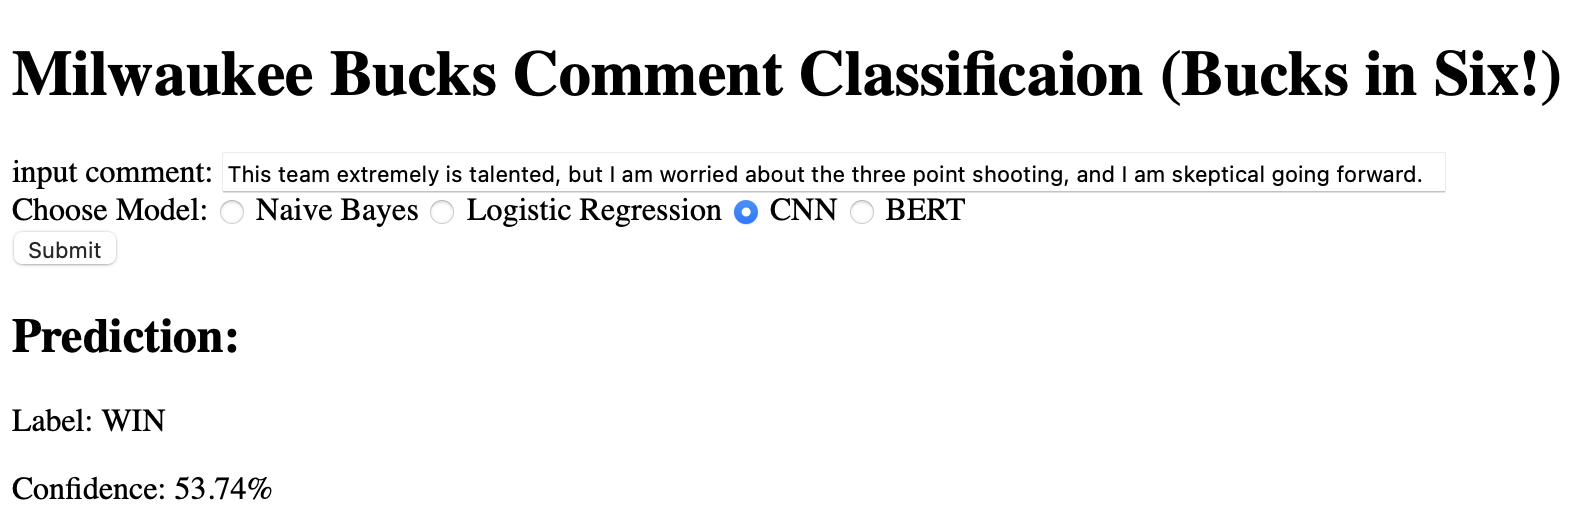
\includegraphics[width=\linewidth]{CNNDEMO.png}
    \caption{CNN Demo}
\end{figure}

The BERT model classifies this comment as a "Win" with "Confidence" = 73.91%.

\begin{figure}[H]
    \centering
    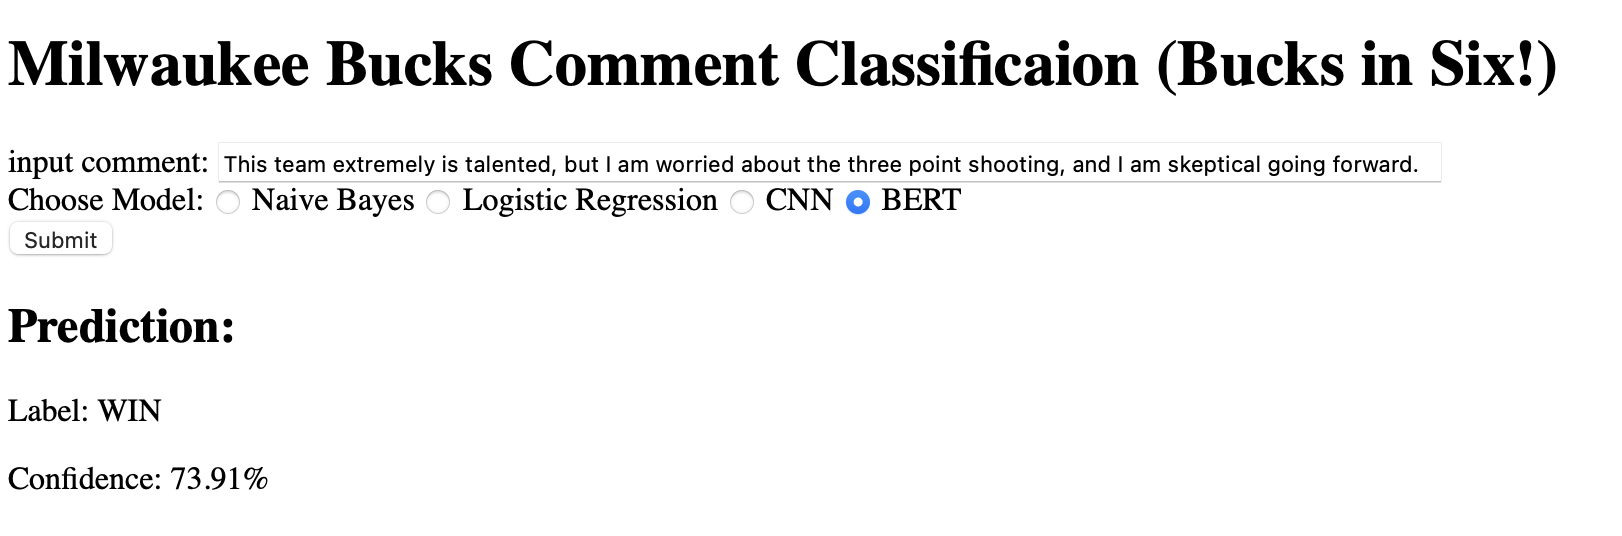
\includegraphics[width=\linewidth]{BERTDEMO.png}
    \caption{BERT Demo}
\end{figure}

Interestingly, only the Logistic Regression classifies this comment as a loss, but only slightly. The BERT model most strongly asserts that this comment follows a win, with the Naive Bayes close behind. The CNN only slightly predicts a win.

\end{document}



